\chapter{不等价结构的生成和查重及其应用}\label{chapter:unique}

通过第一性原理来计算和预测材料的热力学稳定构型是计算材料学近几十年的一个重要发展。
它被称作晶体结构预测问题(CSP),
因为计算过程的自由度和搜索的空间十分巨大,基态稳定结构等结果往往来自对大量的材料构型进行计算,
同时又因为第一性原理的能量计算对计算资源消耗大,要解决CSP问题并不容易。
尽管如此,由于CSP问题有重要的应用价值,吸引了许多的研究关注,
针对这一问题,近些年也发展了非常多的方法。

这一章我们主要介绍CSP的子集,即在晶格类型已知的构型中的晶格衍生结构预测的算法和实现。
虽然是原问题的子集,但它同样非常重要,实验发现许多半导体或金属间形成的合金都是通过这种固定的晶格的形式形成合金。
我们通过自己编写的软件实现了产生不等价的构型,并将这个方法用到了本论文的相关工作中。
枚举产生的不等价的结构产生后会进一步进行结构的优化到达势能面的局域极小值点,
再对比这些局域极小值点的结构的能量,以得到最稳定的构型,从而用于确定热力学稳定性的搜索过程。

\begin{figure}
  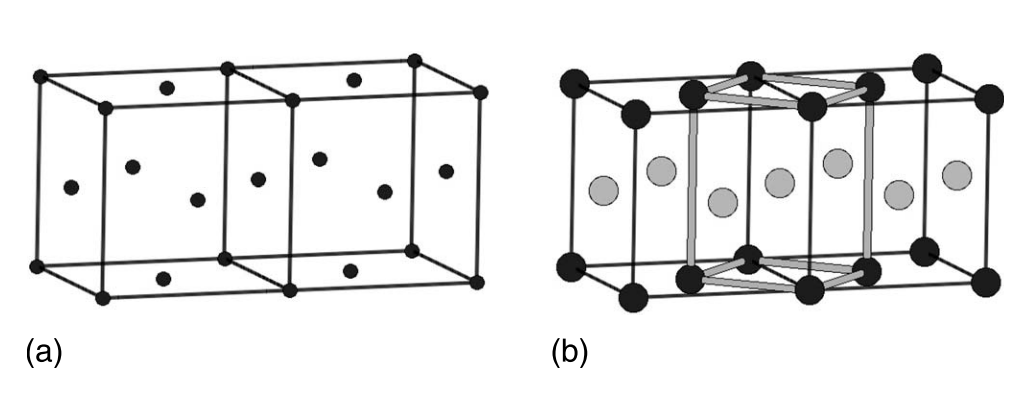
\includegraphics[width=0.72\textwidth]{figs/ch4_fcc_superlattice.png}
  \centering
  \caption{左边是原面心立方晶格,右边是原晶格扩充的超晶格,超晶格是由灰色的双单元格定义的。
  超晶格的两个内部点被一个紫色原子和一个绿色哦原子所占据。超晶格和原子一起构成了一种衍生结构。
  这个例子的所对应的真实合金是\ce{CuAu}合金。}
  \label{fig:ch4_fcc_superlattice}
\end{figure}

\section{构型查重算法概述}
合金中的化学序结构,磁性材料中的磁序结构,
以及非化学配比的带有缺陷序的材料表现出各种不同的性质
都与其原超结构的衍生结构\cite{buerger1947derivative, santoro1973coincidence, santoro1972properties}
有关。同样的还有超晶格的衍生结构,它是孪晶中影响结构和性质的重要因素之一。
那么什么是超结构的衍生结构呢?这里我们定义其为单胞是其原单胞数倍拓展而来,
原子坐标的基矢是原单胞对应的向量加和,但原子排列不同于原单胞的构型。
比如许多金属间化合物可以认为是由\ref{fig:ch4_fcc_superlattice}(a)面心立方晶格衍生而来的超结构,
如图\ref{fig:ch4_fcc_superlattice}(b),构型中的原子占有面心立方晶格所处的原子处,
但因为其有两种原子所以不再有面心立方的对称性,
而成为图\ref{fig:ch4_fcc_superlattice}(a)面心立方结构的衍生的超结构。
图\ref{fig:ch4_fcc_234_ss}中展示了面心立方晶格当超胞晶格体积为单胞的两倍、三倍和
四倍时,所能取得的各种衍生超结构。
在这17种二元面心衍生构型中,所有的二倍和三倍于原晶胞的结构都有实际的物理材料的对应。在四倍的超晶格中,
构型$L1_2$,$B11$,$NbP$和$D0_{22}$四种具有实际的物理材料对应。
\ce{AgPd3},\ce{AgZr},\ce{Pt3Tc}构型已经被文献\cite{curtarolo2005accuracy}预测存在,
但还没有被实验合成。剩余五种构型暂时未被观测或预测存在于任何系统中的。

\begin{figure}
  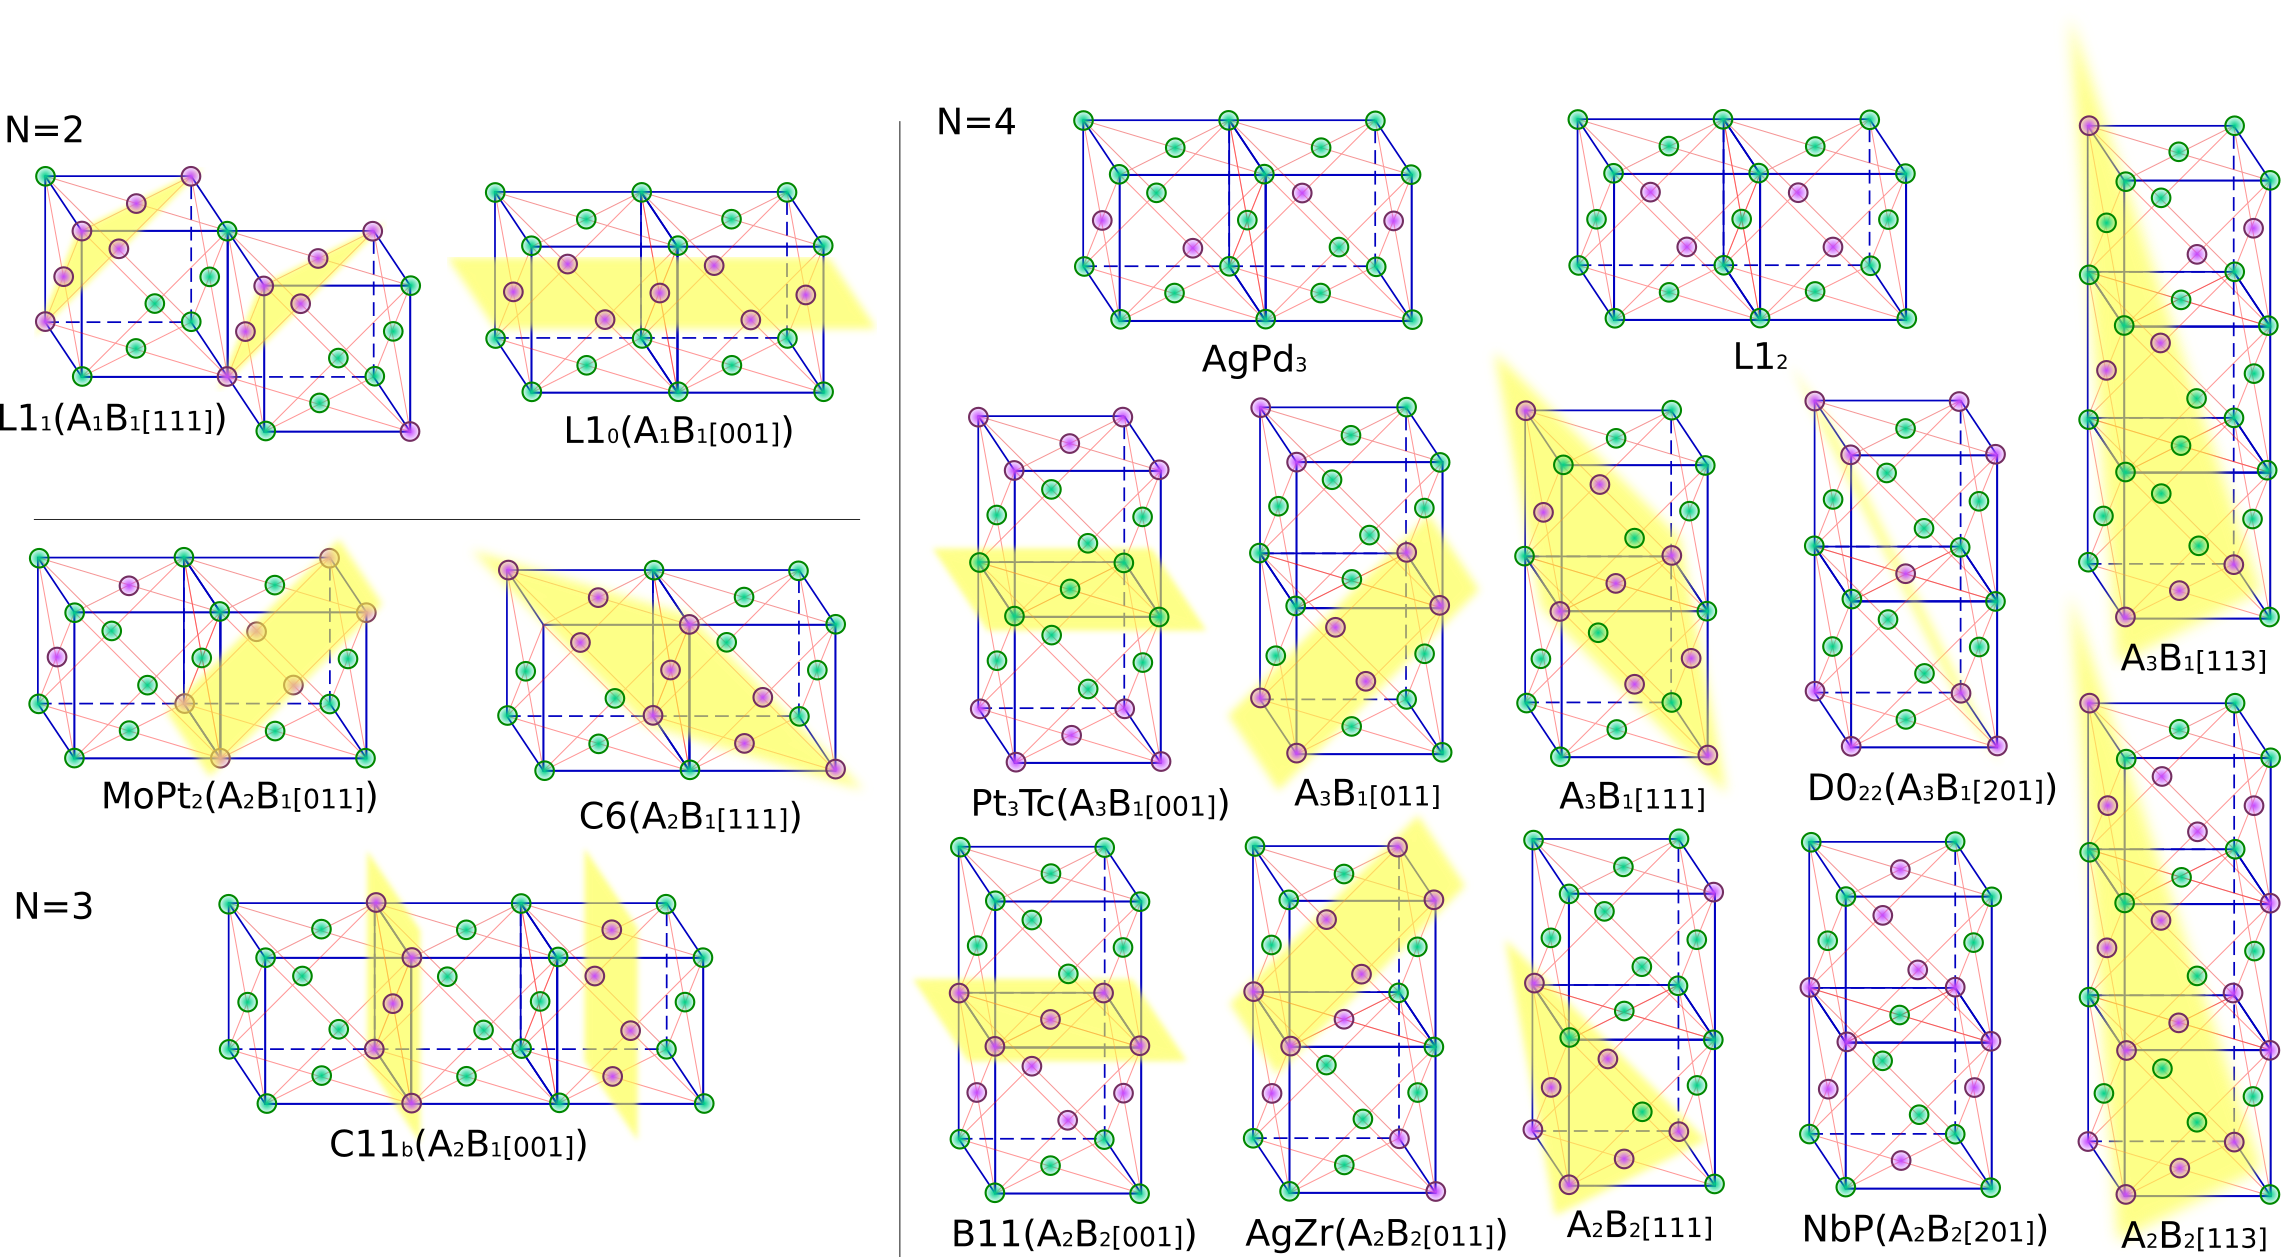
\includegraphics[width=0.96\textwidth]{figs/all17fcc.png}
  \centering
  \caption{面心立方晶格的前17种二元结构。
  超胞体积胞为原胞的二倍三倍或四倍。部分构型可以看作由纯A和B原子层叠加而成。
  例如,左上角的$L1_{0}$结构是一个交替的\ce{A1B1}层序,沿[001]方向堆叠。
  所有的二倍和三倍于原晶胞的结构都有实际的物理材料的对应。在四倍的超晶格中,
  部分构型具有实际的物理材料对应。部分构型已经被文献\cite{curtarolo2005accuracy}预测存在,
  但还没有被实验合成。还有部分构型是从未被观测到或预测存在于任何系统中的。}
  \label{fig:ch4_fcc_234_ss}
\end{figure}

生成的衍生结构的集合通常会被用于如确定固定晶格的二元金属间合金的基态性质。
同时该方法也不仅限于搜索构型的能量,只要能够定义和有序构型有关的哈密顿量,
就能描述其他的物理性质,比如Graf等人\cite{graf2005direct}通过定义经验赝哈密顿量来直接预测半导体合金的带系和费米能级处电子的有效质量。
只要所需要的物理性质和衍生结构构型是有关联的,
就可以通过这种构建赝哈密顿量方法来建立构型和性质的联系从而搜索并预测合金的性质。

为避免重复的计算,我们需要获得衍生结构的集合(数学上的集合概念的推广,该集合中任意两个构型物理上是不等价的)。
构型和构型之间的几何表示可能并不相同,但由于晶体结构的对称性,两种不同表示的结构可能会是物理上等价的,
论文本章的后续章节就是描述了解决这一问题的算法,我们将解决这一问题的算法统一称为枚举查重算法。
我们先简要概述所用到算法的逻辑框架,再在以下小节详细叙述算法细节。
我们采用的枚举查重算法分为两步:
\begin{enumerate}
  \item 晶胞的查重,即产生不重复的超胞。
  \item 对特定超胞进行构型的查重,即产生不重复的编号(即在晶胞对应的旋转和平移操作后不重复的编号)。
\end{enumerate}

第一步晶胞的查重是通过使用厄米标准型(HNF)的整数矩阵来表示由基础单胞扩充而来的超胞,
从而由厄米标准型的唯一性来表示并避免周期性对称下相同超胞的不同表示所造成的重复。
我们首先对给定的行列式值(代表超胞的体积)产生所有的厄米标准矩阵。
因为物理上晶体具有旋转的对称操作,这时所给出的所有矩阵所对应的超胞有部分是可以通过旋转操作等价的。
我们需要再通过对比旋转操作后的晶体的等价性,来去除所有重复的超胞,使每一种超胞仅有一个代表结构。
如图\ref{fig:ch4_2d_square_lattice}所示,
(a)中是所有可能的厄米标准型矩阵对应的超胞,(b)是去除物理等价的超胞后的不等价的超胞。

\begin{figure}
  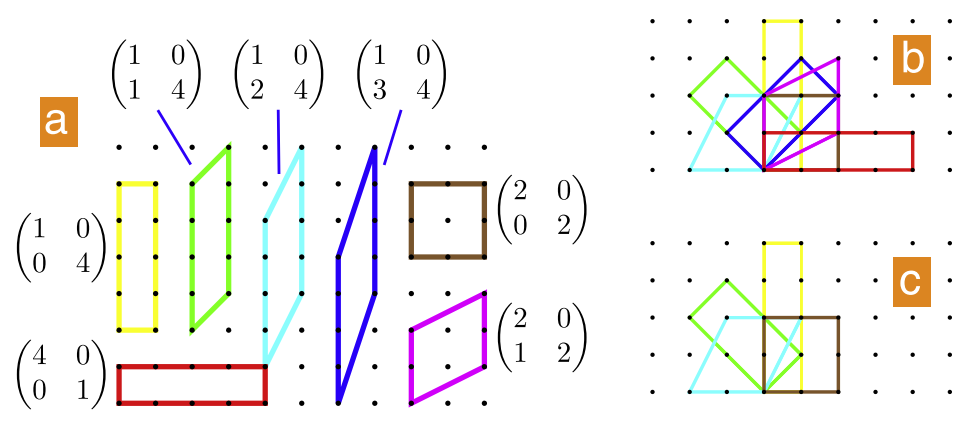
\includegraphics[width=0.96\textwidth]{figs/ch4_2d_square_lattice.png}
  \centering
  \caption{正方晶格:(a) 7个大小为四倍原晶格的厄米标准型(HNF)基矢量及其对应的单位晶胞。
  (b)相同的超晶格,但使用最短的(正交的)基向量来描述。因此这七个二维晶格去重后可以得到四个完全不等价的超晶格。}
  \label{fig:ch4_2d_square_lattice}
\end{figure}

第二步对于特定的超胞,格点位置可以放置不同的种类的原子构成不同的构型,
要判断两个构型之间是否相同,可以通过对一个构型施加其构型对应的所有操作后,
再对比另外一个构型以检查这两个构型是否等价。
在实际操作中,对结构直接作用对称操作得到新的空间坐标的计算效率并不高,
因为针对的是确定格点的结构,格点间的距离这个参数
不会影响等价性的结果,因此可以在构型描述时对所有构型使用统一晶格参数,
再对特定超胞的不同晶格进行编号,
则超胞的商群中的每一个对称操作都会等价于一个置换操作。
以二元合金为例,每个构型都可以由一个二进制「0,1」编号表示,
因此可变换对应于一个十进制整数,
每一个对称操作所产生的效果仅仅是将一个整数变为另一个整数,
我们通过哈希表来储存所有无法通过对称性变换到集合中其他对象的所有非等价的对象。

\section{晶胞的查重}
晶胞查重的第一步是给出所提供的原始晶格的所有表示不等价超晶格
(可包含因旋转操作而重复的晶格),
即产生所有的衍生晶胞的初始非平移等价的有限数量的集合。
我们考虑$B=A\cdot H$,这样的晶胞变换,其中$A$是原始晶胞的基矢
(为表述清晰,论本表述中使用列向量的形式,
所以变换矩阵$H$右乘于原基矢向量。在
但在程序中有时会使用基矢矩阵转置后变为行向量,来表示晶胞的基矢),
$H$为作用在原始矩阵的变换矩阵,其元素为整数,$B$则为变换后的基矢。
如果$H$是一个行列式为\num{+-1}的矩阵,则变换后的晶胞与原晶胞物理等价,
$A$和$B$仅仅是同一套晶胞对应的不同的基矢选择。
换言之,如果整数$H$矩阵的行列式为\num{2},则晶格$B$是晶格$A$的超晶格,
且为单胞体积其原晶格单胞体积的两倍。

我们设有两个整数矩阵$H_1$,$H_2$,它们有相同的行列式值,
如果$H_1$能够通过整数的列操作(列之间的线性运算)变为$H_2$,则他们产生的是同一套晶格。
我们将这些操作矩阵的正则形式表示为下三角矩阵的厄米标准型形式,
这样能够保证每个超晶格都有且仅有一个矩阵对应(下三角厄米标准型的唯一性\cite{santoro1973coincidence})。
三维情况下,下三角矩阵厄米标准型为:

\begin{equation}\label{eq:hnf}
  \begin{pmatrix}
    a & 0 & 0 \\
    b & c & 0 \\
    d & e & f
  \end{pmatrix}, \qquad
  0\leq b < c, \qquad
  0\leq d, e< f.
\end{equation}

这种表示下,矩阵的行列式的值为对角线元素的乘积$a\times c \times f$。
同时,该行列式值$n$也是拓展后超晶格的体积,即将原始晶胞体积看作\num{1}时变换后的单胞的体积倍数。
在这样的定义下,所有的原始晶格的超晶格对应的变换矩阵$H$,都能够通过指定行列式的值后,
将行列式分解为三个整数的乘积形式,再通过式(\ref{eq:hnf})来限制$b$,$d$,$e$的值,
从而构造能将原始晶格变换为超晶格的唯一平移不等价的变换矩阵$H$。

综上,给定$H$矩阵的行列式值后枚举所有的$H$矩阵的算法非常简单:
首先,找到$H$行列式的其中一个因数$a$,
并保证$1\leq a \leq |H|$,
再使第二个对角线因数$c$满足$1\leq c\leq |H|/a$,
最后计算$f$并使其满足$1\leq f\leq |H|/(ac)$。
我们以行列式为$n=6$时的变换矩阵为例,共可以得到如下表中的所有对角线元素$a$,$c$,$f$的组合。

\begin{table}
  \centering
  \begin{tabular}{c|ccccccccc}
    a & 1 & 1 & 1 & 1 & 2 & 2 & 3 & 3 & 6 \\
    \hline
    c & 1 & 2 & 3 & 6 & 1 & 3 & 1 & 2 & 1 \\
    \hline
    f & 6 & 3 & 2 & 1 & 3 & 1 & 2 & 1 & 1 \\
  \end{tabular}
\end{table}

在程序中可以通过简单的二重循环来实现,
分别给出$a$,$c$,$f$的值。
在确定对角线元素后我们需要再确定满足条件的$b$,$d$,$e$所有可能的组合。
同样这一步也能通过嵌套的三个循环来列出符合条件的$b$,$d$,$e$的值的来完成。
通过生成超晶格后统计数量发现,
对于行列式的值为$n=|H|=1,2,3,4,\cdots$的HNF矩阵,
其数量为数列:$1,7,13,35,31,91,\cdots$,该数列满足:

\begin{equation}
  \sum_{d|n} d\sigma(d) = \prod^k_{i=1}\left( {\frac{(p_i^{e_i + 2}-1)(p_i^{e_i + 1}-1)}{(p_i-1)^2(p_i+1)}} \right),
\end{equation}
其中$\sigma$为除数函数求和\cite{erdiis1952distribution},
$p_i$和$e_i$为$n$的因数和幂次,
满足$n=p_1^{e_1}\cdot p_2^{e_2}\cdots p_k^{e_k}\cdot$。

有了明确的数列表达式我们可以验证算法的准确性。
同时还需要强调的是,该HNF矩阵的数量是不依赖于原始晶胞的具体形式的,
即对所有晶胞都适用。但是这里列出的矩阵仅仅是平移不等价的,
针对特定的原始晶胞,在空间中还存在旋转不变形,
我们需要去除旋转变换后物理等价的晶胞。而这需要先验知道晶胞的旋转对称操作的信息。

旋转操作仅仅会改变单胞在空间中的朝向,而不会改变晶胞的形状,
所以两个形状不同的晶胞一定是非旋转等价的。
为了对比形状,可以对晶胞采取了Niggli变换\cite{kvrivy1976unified,grosse2004numerically}变为Niggli标准形式,
从而可以直接对比变换后晶胞之间的形状,去除旋转等价的晶胞。
另外一种去除平移不变形的方法\cite{hart2008algorithm}是通过
对HNF矩阵作用后产生的超晶格作用原晶格所拥有的旋转变换$R$,
若所有旋转操作均不能使两个晶格重合,则确定这是两个不等价的晶格。
在程序中我们选取了两种方式结合的方法来选取不等价的晶格,
即首先通过Niggli变换为形式规范的晶胞(Niggli变换后的晶胞的基矢和基矢夹角有确定的大小排列顺序),
如果旋转对称操作数量不多我们则作用全部旋转操作查重,
如果对称操作过多而候选结构不多,则使用对比每个结构的晶格参数来查重。
效率(时间复杂度)上这个方法并没有很大的优势,
但是可以确保最后给出的超晶格(操作中是变换格点位置放置不同原子的构型,
否则会都变换到统一的原始的晶胞,因为如果不区分格点的元素,
则所有晶格都是相同的)都是统一的Niggli变换后的形式,
使得后续的处理(格点排列的查重以及后续计算提交)更加简洁。
同时,我们还实现了对二维结构的超晶胞的生成和拓展,
独立为软件包pniggli\cite{pniggli}。本文的研究对象是二维材料,
因此会到了这个对二维拓展的工具。

\section{晶体构型的查重}
晶胞的不同是合金材料多样性的基础,如果所有晶格点都是同一种原子,
则即便是不同的超晶格也是等价的。
所以更重要的是,给定超晶格后,在格点放上元素种类不同的原子,产生新的构型。
然而,在摆放上不同原子后,两种构型之间还是有可能经有晶体所拥有的空间群的对称操作互相等价。
因此,这一步晶体构型查重的目的是对于给定晶胞,在晶胞格点位置放置原子后,生成所有不等价的构型的集合。

假定我们选定了一个HNF矩阵,则就拥有了其对应的超晶格,
即一个包含三个矢量的基组以及原子各放置的格点。我们要将$k$种元素放置在格点上构成特定构型,
格点标记为$a,b,c \cdots$。
HNF矩阵描述了晶格的体积为$n$即有$n$个格点。
预将k种元素放在$n$个格点上共有$k^n$种不同的放置方法,
但其中的许多摆放方法因为晶格的空间对称性,其两两之间是物理等价的,
为了描述每个构型,我们将每种放置方法对应为一种编号。
合理的编号方法不但方便了描述,还能带来了算法上的加速。 
为了简化算法的描述,在本节中
我们仅以原始晶胞中包含一个原子的格子为例,
比如面心立方和体心立方的原胞格子,
而不是六角密堆的格子其原胞中包含两个不等价的位点。
本节所叙述的方法可以容易地拓展到如六角密堆的格子中\cite{hart2009generating}。
拓展到一个原始晶胞包含多个原子,仅仅只是表述上更加复杂,
在算法上基本上是完全等价的,我们的软件上实现的是对原胞中包含任意个数原子的晶格的拓展。

晶格的不同位点上可以摆放各种各样的原子,形成不同的晶体构型,
晶体构型的查重问题,就是在所有的$k^n$种结构中选取唯一的不与其他构型等价的构型的问题。
我们以如图\ref{fig:cell-undup}的$2 \times 2$的二维正方格子形成\ce{A2B2}化合物为例。
该二维晶胞共有四个原子位点,若要构成\ce{A2B2}化合物,
则共有${4\choose 2}=6$ 种构型。
但根据平面二维正方晶格的平移和旋转对称性,仅有如图\ref{fig:cell-undup}(b)、(c)的
两种是不等价的。
如图\ref{fig:cell-undup}(c)、(d)两种,可以互相通过晶格的
旋转和平移操作得到。
因此仅有两种不等价的构型。

\begin{figure}[htb]
  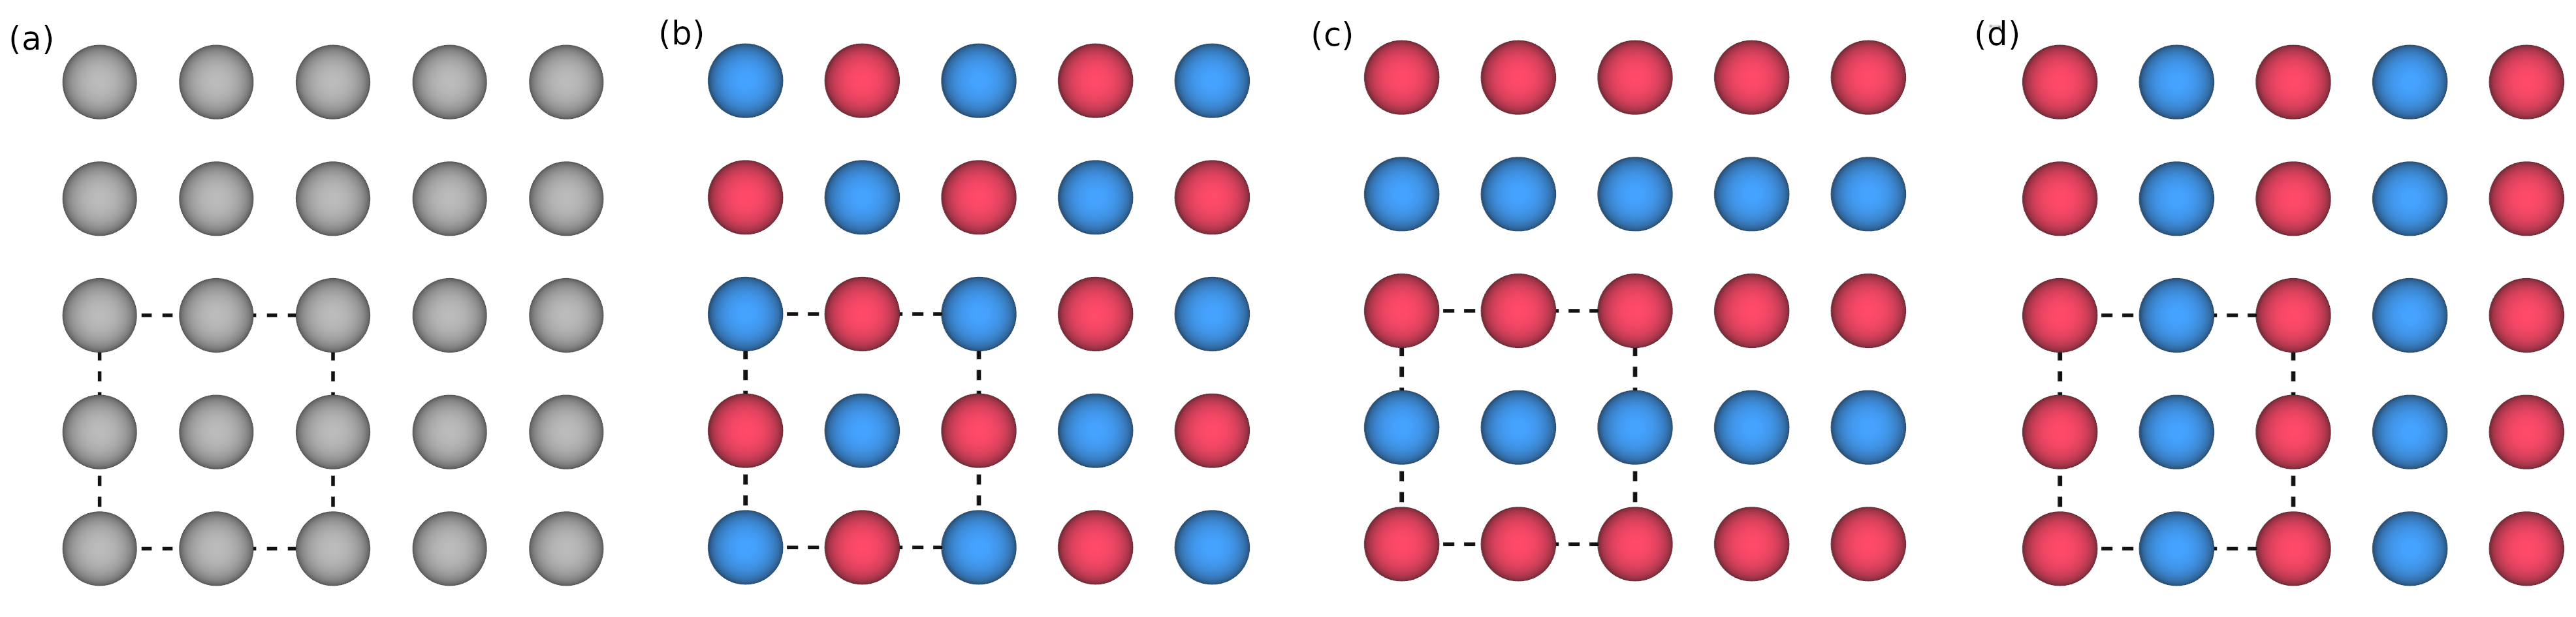
\includegraphics[width=1.0\textwidth]{figs/cell_undup.png}
  \centering
  \caption{(a)晶格位点未放置具体原子。(b)(c)(d)三种可能的放置方式,其中(c)、(d)是两种等价的构型}
  \label{fig:cell-undup}
\end{figure}

早前在上世纪90年代,Ferreira等\cite{ferreira1991stability}实现了FWZ算法来完成这以目的,
他们算法是简单的对比任意两个构型,
通过作用所有的对称操作来确定是否能由其中一种变换为另外一种,
从而判断其等价性。该方法实现上非常直观,但因为要两两对比结构,
其时间复杂度为$\mathcal{O}(N^2)$。
我们在软件中使用了数据结构层面改进的
源自Hart等在文献\cite{hart2008algorithm}中,描述的基于群论的方法来去除不等价的构型的算法,
从而实现时间复杂度为$\mathcal{O}(N)$的查重操作。
其时间复杂度下降的原因归纳来说,
就是对所有构型进行晶胞(从原始晶胞变换扩充后,但格点上还没有区分放置的原子)所拥有的对称操作,
从而得到每个构型所对应的衍生结构,
所有的结构和衍生结构都通过对应的编号表示(编号表示影响的是后续查重的单步时间以及数据存放所占用内存的大小)。
再将所有构型(编号表示)进行哈希表的储存,从而仅存放构型不同的对象,
构成一个集合(数学上集合的概念,即元素之间不重复)。
对每个构型所做变换得到新的表示的个数为晶胞的对称操作数量。
但实际算法中,并不需要作用全部的对应空间群中的全部操作,后面我们会看到,
借助史密斯标准型表示衍生后的晶格,
具有相同商群的晶格可共享一套编号而一次性进行平移对称性的查重,
这会使得算法在效率上获得进一步提升。

对构型进行编号的主要作用是:
\begin{enumerate}
  \item 所有构型共用一套格子,通过编号可以节约对构型信息的储存。只需要原始晶胞(格子类型)和HNF矩阵(超晶胞)加上编号就能够还原一个特定构型。
  \item 通过编号,一个构型可以将对构型的一个空间群所拥有的对称操作映射为对应的一个对编号的置换操作,这使得对构型的单步变换操作变得更快。
\end{enumerate}

以三维晶体的结构查重为例,
我们来描述如何通过对晶胞格点进行编号来进行查重操作。
设拥有一个原始晶胞$L$以及通过H矩阵扩充后的超晶格$S$,
$S$是$L$的一个子群(这是显然的,因为$S$的所有群元操作都可以作用在$L$上)。
以一种对$S$具有周期性的方式标记$L$等价于仅仅标记商群$G=L/S$的元素。
需要注意,因为平移周期性,$L$和$S$有许多种标记方法,但其商群$G$是固定的。
与晶格的查询相似的是,我们并不对晶体作用平移操作,
而是在其所属的群中进行全部群元操作来查重。
具体实现中用到了变换矩阵的史密斯标准型(SNF),
即HNF矩阵的对角矩阵,其直接提供了超晶格的商群,
SNF的作用是对不同的超晶胞(相同体积扩充后,但不同的HNF矩阵对应的晶胞)
进行一个初始归类,因为SNF矩阵的数量大大少于HNF矩阵,
从而对于有相同SNF矩阵的晶胞,可以采用相同的编号规则的查重,
来一次性去除平移对称操作(即编号的轮换操作)所导致的重复,
从而大大减少对每个结构所需要的对称操作数量,因此能够大大降低整体的运行时间。
这是因为,SNF矩阵的作用是和编号息息相关的,
对于对应相同SNF矩阵的不同HNF矩阵的超晶格,
可以共用一套编号方式以及该编号下晶体对称操作映射的对编号的置换操作。

之后,在对一套格子编号后,
我们需要对编号进行等价性的判断,
仅保留对应唯一不重复构型的编号。其中需要排除的是:
\begin{enumerate}
  \item 编号的轮换对称操作后等价的构型(因为编号本身不影响构型),其实该操作就是前面同类SNF矩阵对应晶胞的平移操作后的等价查重
  \item 编号的交换对称(编号本身不影响构型)
  \item 编号后可缩减为更小的超胞(该条件仅用于已经在较小体积的超晶格中已经统计了这个构型)
  \item 由于晶格旋转对称操作导致的编号置换。
\end{enumerate}
其中前两种属于相同情况,我们在编号的生成时就仅仅生成唯一的序列。
针对第三种情况,若一个编号对应的构型能够被缩减为一个更小的构型,
那么该编号在其自身的某一个置换操作下一定会等价于其自己,
通过这个条件我们可以排除这类构型。实际软件的实现中,
我们将这一选项设置为可选,以便用户有时候要仅仅对某一个超晶格来生成所有不等价的构型。
而第四种由于旋转对应的置换操作所等价的编号的等价去除方式与之前的晶格判断类似,
即作用所有的旋转操作对应的置换操作来实现。

\begin{table}[htb!]
  \centering
  \begin{tabular}{cccc}
    \hline\hline
    n(胞体积) & 二元 & 三元 & 四元 \\
    \hline
    2 & 2      &         &            \\
    3 & 3      &     3    &            \\
    4 & 12      &    13     &    7        \\
    5 & 14      &    23     &    9        \\
    6 & 50      &     130    &    110        \\
    7 & 52      &      197   &      211      \\
    8 & 229      &     1267    &      2110      \\
    9 & 252      &     2322    &       5471     \\
    10 & 685      &    9332     &      32362      \\
    \hline\hline
  \end{tabular}
  \caption{面心立方晶格二元、三元和四元衍生物结构的数目。}
  \label{table:derive_structures_num}
\end{table}

需要提到的是,在对结构编号后,对空间构型的操作会变为对编号的置换操作,在程序实现中,我们使用工具spglib\cite{togo2018texttt}来给出所用的对空间构型(超晶胞下而非原晶胞)的对称操作,再对定制编号给出所用对称操作映射的置换操作,并储存成一张表(数据结构上使用一个二维矩阵,每行为一个置换的序列,行数是对称操作的数量)。

至此我们详细描述了构型查重与生成的详细细节,在本章的最后我们给出面心立方晶格,二元,三元,四元下的构型不等价构型数。从表格\ref{table:derive_structures_num}中可以看到当元素种类增加后,构型的数量快速增加。

\section{构型查重在氟化石墨烯构型预测中的应用}

氟化石墨烯(F-graphene)是一种重要的石墨烯衍生物\cite{samarakoon2011structural,leenaerts2010first}。
到目前为止,已经发展了许多合成F-graphene的方法。例如,Nair等人通过将石墨烯暴露于氟化剂\ce{XeF2}中获得了一种衍生物。
所得到的F-graphene是一种优良的绝缘体,
具有很高的热稳定性和化学稳定性,可以用作原子级别的绝缘体或石墨烯基异质结构中的隧道屏障\cite{nair2010fluorinated}。
通过在反应离子刻蚀(RIE)系统中使用可控的\ce{SF6}等离子体处理,
Sun\cite{zhang2016spectroscopic}等人实现了单层化学气相沉积(CVD)生长的石墨烯的氟化,该石墨烯可用于灵敏的氨气体检测。
此外,Yang等人\cite{zhong2016interface}还发现使用\ce{SF6}等离子体处理,也可以在电感耦合等离子体系统中制备F-graphene。
F-graphene作为绝缘体中间层,硅的表面抑制载流子复合,从而实现了高转换效率的太阳能电池。
最近,Hu等人\cite{du2017broadband}报导了F-graphene/graphene 范德华异质结构的宽频带光探测器,
由于$sp^2$杂化的空间不均匀量子限域效应和$sp^3$杂化的局域态光激发载运子捕获的协同导致了宽带隙。
但F-graphene/graphene 光电探测器(PD)的响应速度和响应速度有待进一步提高。

实验中将F-graphene与Si基底结合,能够实现F-graphene/Si异质结器件,该器件具有宽频带光电检测功能,
既可作为光电导电性PD器件,也可作为光电二极管PD器件。
在第一种工作模式下,F-graphene/Si器件在从深紫外光(DUV)、可见光到近红外(NIR)的宽频带光谱区域表现出良好的弱光探测能力,
在\SI{650}{\nm}光下具有\SI{1.9d-7}{\ampere\per\watt}的高响应率(R)照明。
同时,F-graphene/Si异质结具有显著的光伏特性,可以作为自供电的宽频带光电二极管。
在\SI{650}{\nm}光照下,该工作模式的光暗比$I_{\mathrm{light}}/I_{\mathrm{dark}}$为\num{2.0d-5},
响应速度$(\tau_r/ \tau_f)$为\SI{6.3/9.7}{(\us)}。
第一性原理计算揭示了F-graphene的带隙随F原子覆盖度的变化,揭示了紫外和近红外区域响应率显著提高的原因。
这种双模PD可以同时实现弱光检测和快速光检测,克服了传统单模PD的局限性。

为了研究实验中用等离子体处理CVD生长石墨烯的氟化过程,
我们通过的结构生成和查重算法给出实验上可能的F-graphene构型,
并对给出构型进行能量和电子结构的第一性原理计算。
为了模拟非全覆盖氟化石墨烯的性质,我们使用了 $2\times 2\times 1$ 共有8个碳原子的超胞。
对于给定的石墨烯单元,每个氟原子可以石墨烯的两侧在与碳原子成键,根据一个碳原子和氟原子的成键数,分为三种情况:

\begin{enumerate}
  \item 碳不与氟键合
  \item 氟原子在石墨烯平面上方与碳成键
  \item 氟原子在石墨烯平面下方与碳成键
\end{enumerate}

我们不考虑一个碳原子上下都附着有氟原子的情况,因为这时的碳原子将不再满足四配位结构,能量上不占优。
但即便有这个结构限制前提条件,所可能的氟化石墨烯构型数量还是巨大的。
为此,我们本小节所介绍的构型的查重在这个计算中是十分必要的。
通过结构查重,我们排除了重复的构型后对不重复的构型进行了高通量第一性原理计算。
若不考虑构型之间的重复,那么每个碳原子与氟原子有三种成键方式,总数为$3^8=6561$,
在经过结构查重后,不重复的构型数减少为\num{267}。
比如,对于氟原子覆盖度为\SI{20}{\percent}的氟化石墨烯,
共有如图\ref{fig:fgr-6}六种可能的构型
这个数量是可以全部进行精确的第一性原理计算来获得准确的能量和电子结构信息的。
同时在查重中还能够给出每个构型在所有\num{6561}个结构中的重复数量,从而我们可以进行后续的热力学性质的计算。
对于全氟化石墨烯,所有碳原子都有一个氟原子键形成$sp^3$杂化。

\begin{figure}[htb]
  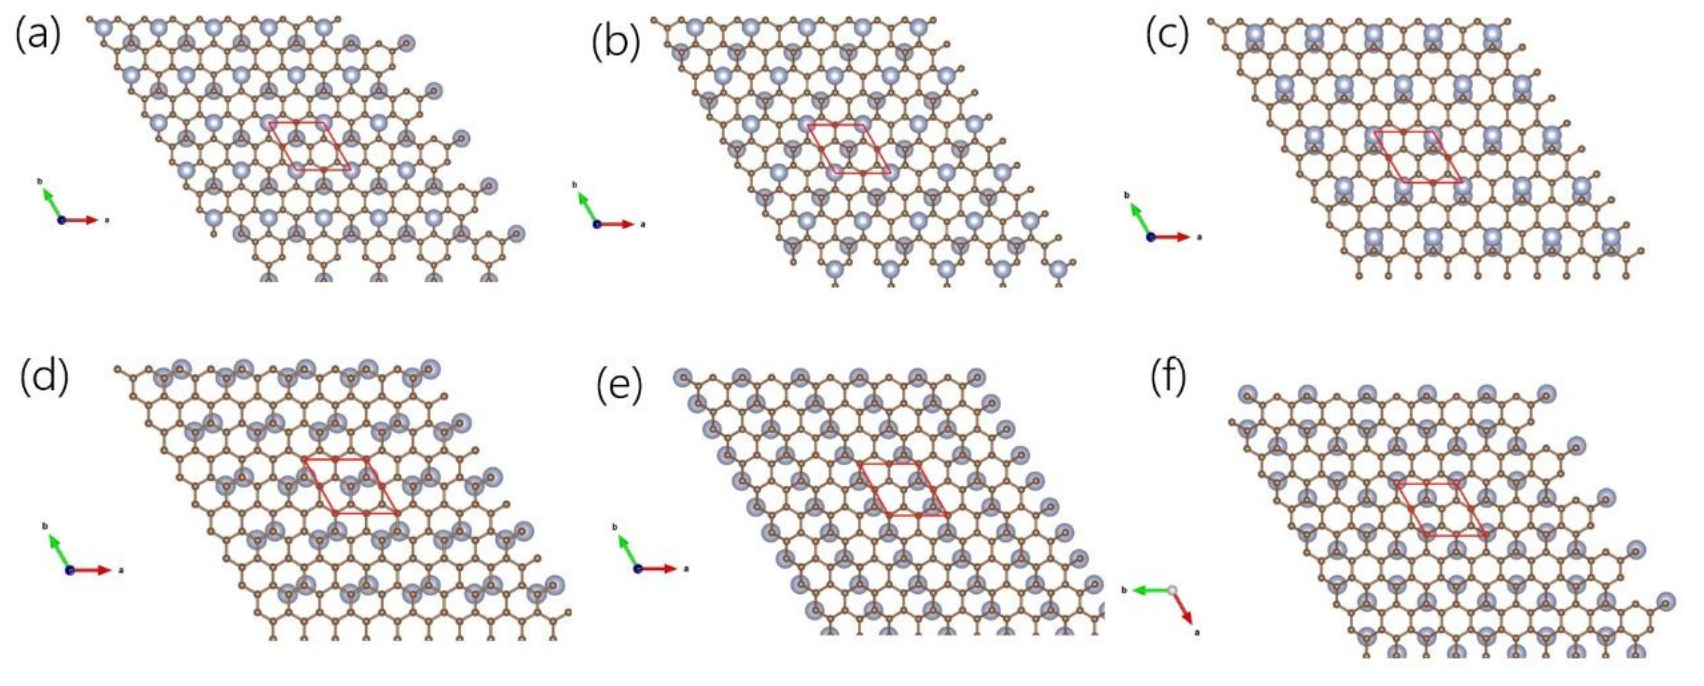
\includegraphics[width=1.0\textwidth]{figs/fgr-6.png}
  \centering
  \caption{氟原子覆盖度为\SI{20}{\percent}的六种可能构型。}
  \label{fig:fgr-6}
\end{figure}

我们发现,对于全氟化石墨烯,椅型结构是最稳定的,与文献\cite{leenaerts2010first}所报导一致。
由于排斥作用,氟原子有在实际空间中分散排列的趋势,这表明所有构型中相邻碳原子所连接的氟原子附着在同一侧的构型能量不占优。
若加上这个额外限制,构型数量进一步减少到35个。
图\ref{fig:fgr-b}中的红点数据为加上额外限制后的35个构型能隙,叉号对应的是不加上氟原子不相邻这个限制查重后所得到
的267个构型。下面不同配比下自由能随温度变化的计算用到的是不加限制的267个构型。
图\ref{fig:fgr-6}分别显示了不同F覆盖下\ce{F_{0.25}C}的六种不同异构体。

就氟化石墨烯,理论计算的意义在于:即便我们的实验结果表明,氟原子能够在石墨烯表面与碳原子形成稳定化学键,
从热力学的角度,在低温时(低于\SI{300}{\kelvin}),计算结果表明,非全氟化-石墨烯的形成却并不是一个自发的化学过程。
我们使用了第一性原理软件包VASP\cite{hafner1997vienna}进行结构的优化和能量及电子结构的计算,
计算中使用了PAW的赝势及方法\cite{blochl1994projector},
交换相关泛函采用PBE形式\cite{perdew1996generalized},
结构驰豫中,放开原子位置和晶胞参数的优化,收敛标准为能量差小于\SI{1d-4}{\eV},
平面波的截断能设为\SI{480}{\eV}。
针对不同结构使用相同的倒空间k点分布,即平均间隔为\SI{0.5}{\per\angstrom}。
给定构型的形成能我们使用如下公式\ref{eq:fgr-formation}计算得到:

\begin{equation}\label{eq:fgr-formation}
  E_{\mathrm{form}}(\mathrm{F_x C}) =
    E(\mathrm{F_x C}) - x E(\mathrm{FC}) - (1-x)E(\mathrm{C})
\end{equation}
其中,$x$为F原子在石墨烯上的覆盖度,$E(\mathrm{F_x C})$、$E(\mathrm{FC})$和
$E(\mathrm{C})$分别为部分覆盖、全覆盖和纯石墨烯的能量。
为了考虑稳定对体系形成能的影响,我们计算体系自由能为:

\begin{equation}\label{eq:fgr-free}
  E_{\mathrm{free}}(\mathrm{F_x C}) = -kT \ln \sum_i g_i \exp (-E_{\mathrm{form}}^i / kT)
\end{equation}
其中,$k$为波尔兹曼常数,$T$为温度,$g_i$为某一覆盖度下特定构型的多重度。

\begin{figure}[htb]
  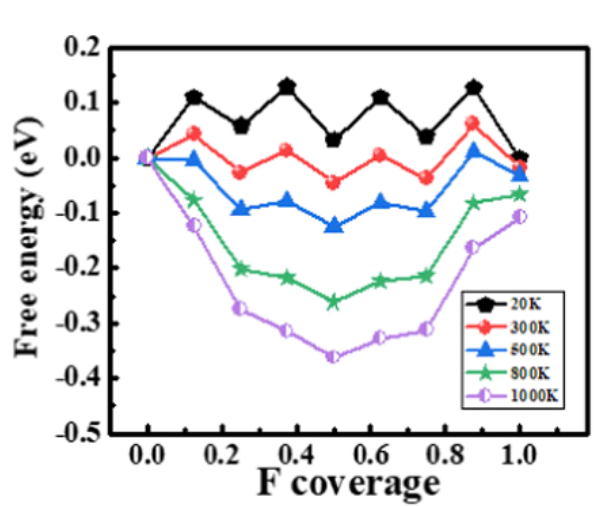
\includegraphics[width=0.5\textwidth]{figs/fgr-a.png}
  \centering
  \caption{不同温度不同浓度F掺杂石墨烯的自由能。}
  \label{fig:fgr-a}
\end{figure}

根据公式\ref{eq:fgr-formation}可以计算得到图\ref{fig:fgr-a},
从该自由能随温度变化的图中可以看出,
在\SI{300}{\kelvin}时,非全氟化-石墨烯的自由能在所有不同的F覆盖率时均在\SI{0}{\eV}附近。
然而,当反应温度增加到\num{500}、\num{800}或\SI{1000}{\kelvin}时,自由能差将大大减小到小于\SI{0}{\eV},
表明在相对较高的温度下发生了自发氟化过程。
可以看到,随着温度的升高,构型熵将使得非全氟化石墨烯的结构稳定性增加,防止其相分离为纯石墨烯或全氟石墨烯,
其中非全氟化石墨烯的结构多样性可能进一步诱导各种光学性质。

\begin{figure}[htb]
  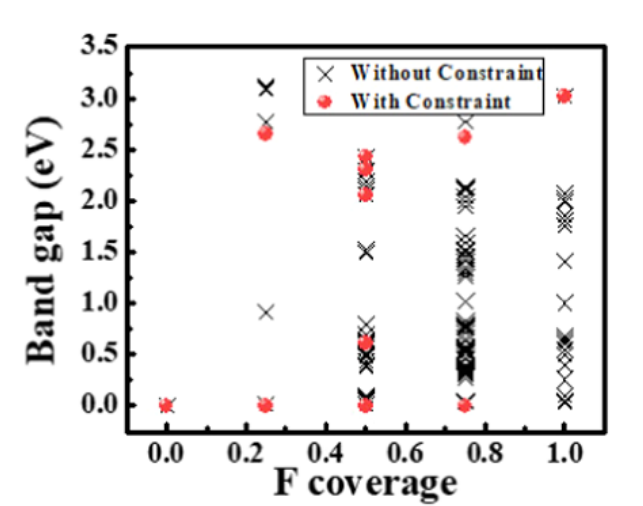
\includegraphics[width=0.5\textwidth]{figs/fgr-b.png}
  \centering
  \caption{不同F掺杂浓度的氟化石墨烯的理论带隙。}
  \label{fig:fgr-b}
\end{figure}

为了揭示F-graphene/Si器件宽带灵敏度背后的原因,我们计算了不同掺杂浓度下F-graphene的能带结构和态密度(DOS)(图\ref{fig:fgr-b})。

结果表明,F-graphene的能带宽度不仅与F的覆盖范围有关,而且与同分异构体结构有关。
无掺杂的graphene带隙为\SI{0}{\eV};然而,当F原子掺杂\SI{20}{\percent}时,共6个不同的构型有不同的带隙,范围从\num{0}到\SI{3.1}{\eV},
对应于不同的异构体结构。

在其他掺杂浓度如\ce{F_{0.5}C}和\ce{F_{0.75}C}上也观察到了类似的带隙打开(图\ref{fig:fgr-cdef})。

\begin{figure}[htb]
  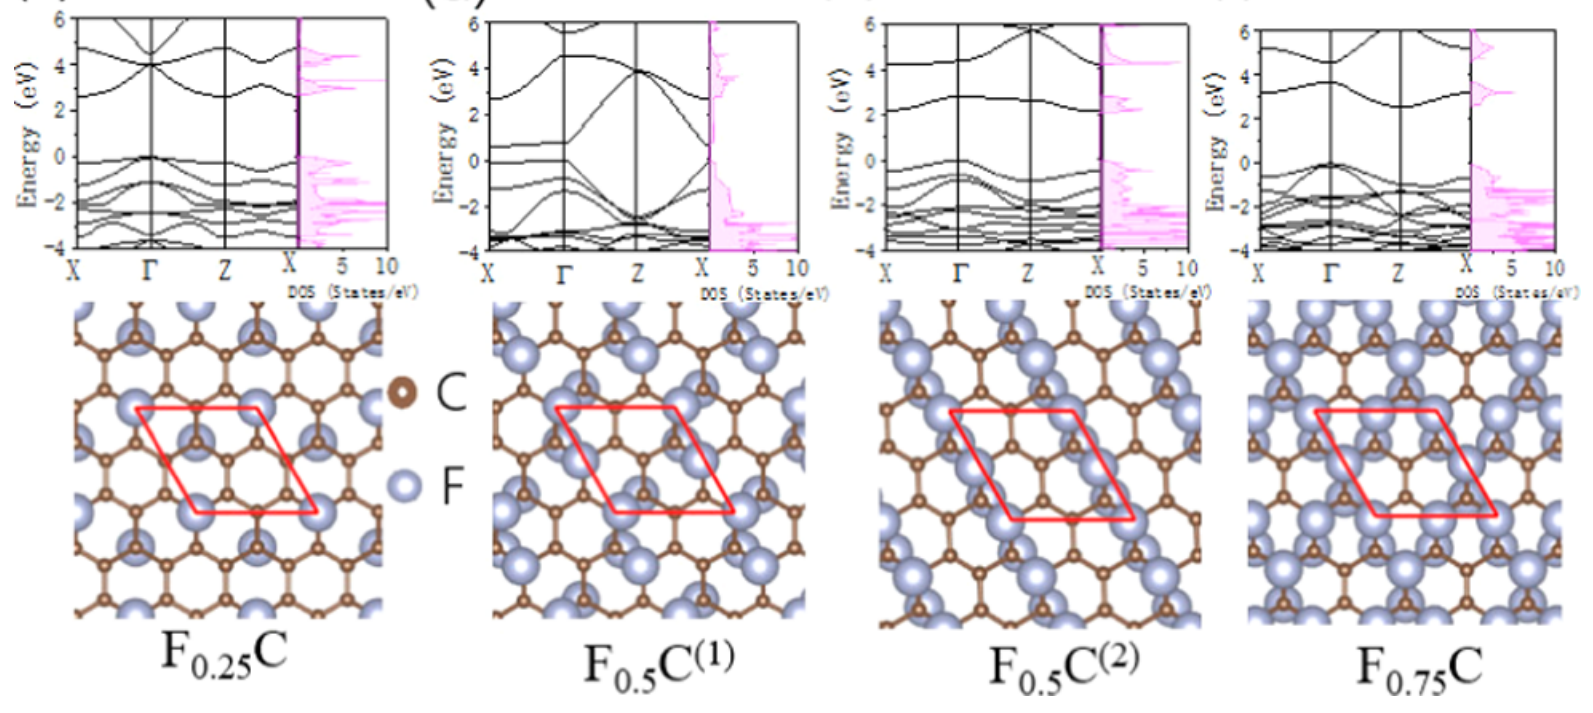
\includegraphics[width=1.0\textwidth]{figs/fgr-cdef.png}
  \centering
  \caption{四个特征浓度的氟化石墨烯的构型和能带与态密度。}
  \label{fig:fgr-cdef}
\end{figure}

考虑到RIE室中氟化的复杂性和F掺杂水平的可控性较差,精确测量F-graphene的微观结构具有很大的挑战性。
尽管如此,我们相信,基于F-graphene/Si的异质结PD在紫外和近红外光谱区域的增强响应是由于氟化导致的带隙增加。
由于氟掺杂的异质性,不同F覆盖度且不同带隙的F-graphene可能共存于F-graphene层。
由于不同覆盖度以及不同的非全氟化石墨烯的构型不同,构型的能带的分布范围较广,
有利于紫外光、可见光和近红外光的宽光谱吸收,导致从深紫外光到近红外光区域的宽带光响应。

\section{单层硼化钛的结构多样性与不等价结构生成}

在绪论部分已经介绍了以过渡金属为中心的多配位硼轮平面团簇能够表现出很好的结构稳定性,
同时结合了已经有理论预测报导的由过渡金属和硼所构成的稳定二维平面结构。
我们因此认为过渡金属和硼能够形成种类多样且拥有新颖优异的物理化学的二维材料。
在本节的工作中,我们选择四周期过渡金属钛作为嵌入硼平面的金属原子,探索其可能出现的稳定平面构型。

在该章所描述的工作之前,有如下一些文献预测报导了钛硼二维材料。
2014年由Zhang等人\cite{zhang2014prediction}预测报导的单层\ce{TiB2}结构,
结构上,钛原子由六个硼原子包围,硼原子形成蜂窝状结构。
该化合物的能带结构中存在狄拉克锥,最大费米速度为\SI{0.57e6}{\meter\per\second},约为石墨烯的一半。
2017年由Qu等人\cite{qu2017two}所报导的单层平面\ce{TiB4}结构,
钛原子由八个硼原子包围组成八配位的钛硼结构,八个硼原子到中心钛原子的距离均相等,
且从侧视图可以看到,整个结构是一个完美的平面,原子之间没有起伏。
2017年Wang等人\cite{wang2017semimetallic}报导了多种二维钛硼平面构型,
构型中的钛硼原子数比从$1:2$到$1:16$,这一系列的构型可分为两大类,
一类为钛硼所组成的单层平面结构,一类为钛原子处在两层硼平面之间的三明治结构。
其中的\ce{TiB12}的能带结构中存在狄拉克锥,通过对该结构施加横向张力,\ce{TiB12}的功函数和电导能够被调控。

\begin{figure}[htb]
  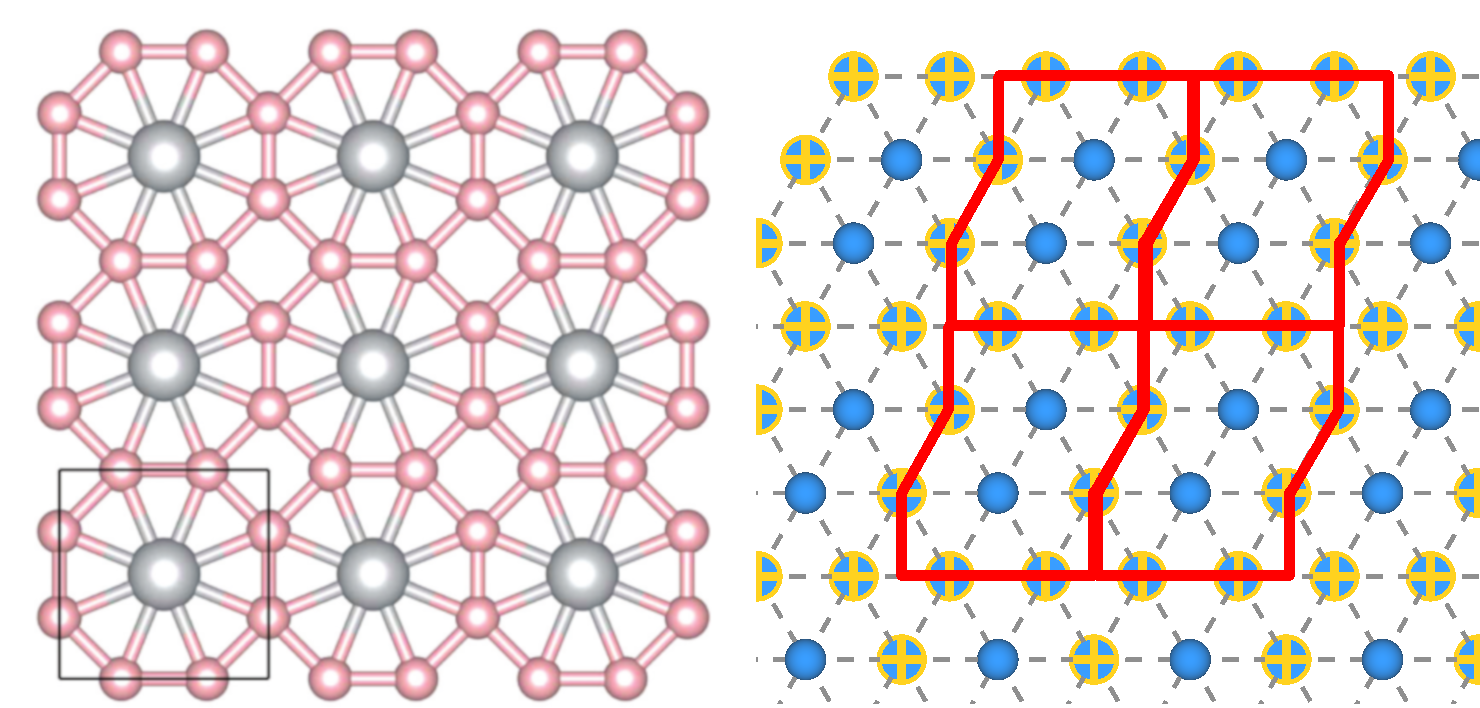
\includegraphics[width=1.0\textwidth]{figs/ch4_cell_change.png}
  \centering
  \caption{从\rom{1}初始构型演变为最后稳定的\ce{TiB4}结构,可将每个硼原子变化前后的位置一一对应。}
  \label{fig:ch4_cell_change}
\end{figure}

需要强调的是,所有已经报导的钛硼二维结构都是通过材料搜索的方法发现的。
全局材料搜索的方法有其一定优势,它只需要极少的起始变量就能对特定化学配比的化合物在势能面上以很高的自由度进行材料搜索。
但也因为自由度过高,搜索过程中所可能经历的构型数量非常巨大,而其中的许多相近的初始结构往往会在结构优化后变为相同的构型,这在一定程度上即浪费时间,也浪费了计算资源。
另外,固定元素之间形成的化合物往往会存在特定的结构特征,利用先验的引入结构特征将能够确定更合理的设置初始构型集合,从而大大减少计算过程中所需要的时间,减少计算资源的浪费。
以二维钛硼结构为例,我们可以发现,稳定的钛硼构型都是由钛为中心,硼环绕的超多配位结构,这也恰好符合硼与过渡金属形成多配位团簇时出现的结构稳定性。

由于钛-硼键的键长和硼-硼键的键长之间存在巨大的差别,
我们认为钛硼不容易出现六配位的结构,比如在过往报导的文献中,
\ce{TiB4}单层是一个全平的平面,其中钛和硼形成八配位的等边多边形,
以及硼硼之间形成的四边形,如图\ref{fig:ch4_cell_change}右边的结构优化后
的\ce{TiB4}所示。因此我们认为该结构是有一个钛原子处于中心的\ce{Ti}@\ce{B8}轮状团簇图案平铺而成的。

以此为出发点,我们将所要探索的二维钛硼结构的集合限制在钛硼单层,
并且钛原子作为中心原子被硼原子环绕。利用这样的初始结构,
我们优化得到了全部已经报导的钛硼单层二维结构,并发现了一些新的具有新颖性质的稳定结构。
我们的计算覆盖了很大的化学配比范围,并基本能够确保包含了所有可能的结构组合。
同时,所需要计算的构型数量也并不很大,通过与高通量工作流工具结合,能够很快完成结构的优化和性质的计算。

硼原子构成硼平面的结构多样性丰富,但结构的区别均体现在空位分布位置的不同上,也就是说,
硼原子网络始终保持为三角格子。过渡金属硼构成的单层平面结构,
过渡金属均采取多配位的结构,同时硼网络均能够看做是三角各自轻微程度扭转而成的,
如图\ref{fig:ch4_cell_change}所示,我们展示了如何从初始构型结构优化过程中通过胞和
原子的轻微位置变化获得新的稳定结构。利用这样的结构上的特征,
我们选择在硼原子构成的三角格子网络中用过渡金属原子嵌入网络并替换一个或多个硼原子来构造初始平面单层钛硼网络。
这样在结构优化过程中,原子仅仅在原始位置周围移动调整网络的空间结构,
即保证能够在势能面的每个可能局域极小值附近都有初始构型,从而对势能面上的所有局域极小结构进行遍历,并考察结构稳定性。


\begin{figure}
  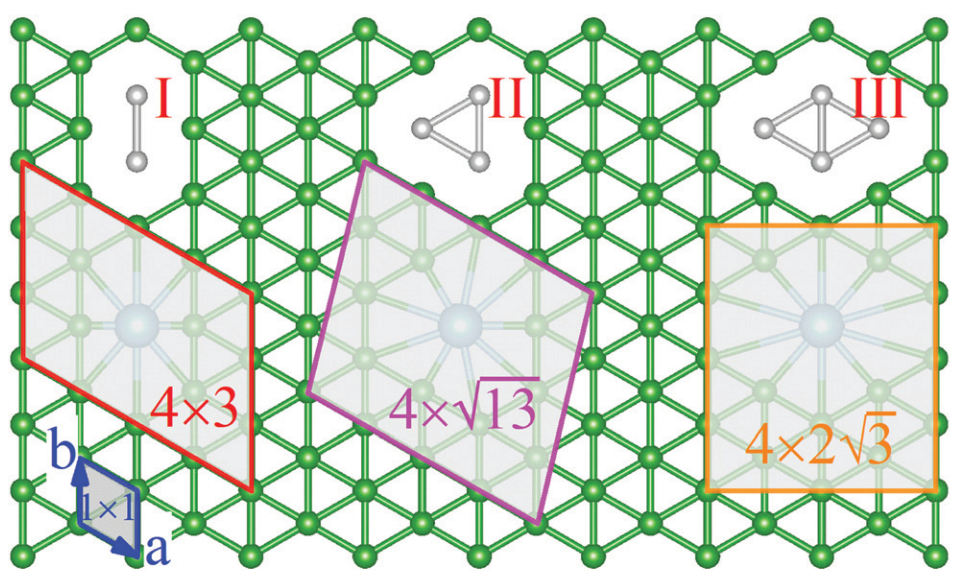
\includegraphics[width=1.0\textwidth]{figs/ch5_how_cell_choose.png}
  \centering
  \caption{单层硼化钛的结构生成示意图。在\rom{1}型、\rom{2}型和\rom{3}型中,一个钛原子分别替代两个、三个和四个硼原子。蓝线勾勒出的菱形表示二维三角晶格的单元格。还同时显示了超胞。大的天蓝色球和小的绿色球分别代表钛原子和硼原子。灰色的球代表要被取代的硼原子。}
  \label{fig:ch5_how_cell_choose}
\end{figure}

之前文献报导的二维\ce{TiB2}化合物为三明治夹层结构\cite{zhang2014prediction},
硼原子形成两层硼平面,钛原子在两层硼平面中间作为插层并与周围的硼原子成键,
其中钛原子与硼原子之间的距离为\SI{1.19}{\angstrom}。
类似的过渡金属-硼构成的三明治夹层结构在其他的钛硼、铁硼二维结构中也由发现。
而我们的工作,我们将搜索的结构范围限制在单层钛硼结构,
旨在探究钛原子与硼形成单层的钛硼平面,并对比所有这类单层平面的结构稳定性。
同样的方法可以很容易地拓展到三明治夹层结构的结构预测中。

为得到这样的单层过渡金属硼平面,我们按照如下的方法来构建初始构型。
首先,确保硼原子按照三角格子密堆的形式形成硼单层网络,其次,在网络中插入过渡金属钛原子与硼成键。
然而,由于过渡金属的半径较硼的大得多,其原子很难只是通过替换单个硼原子,
来与硼原子网络中的其余硼原子通过六配位的方式来嵌入硼原子网络中而形成二维钛-硼单层结构。
根据过渡金属与硼形成轮状团簇时实验观测到的都是多配位的团簇这一结论,我们认为,
在单层过渡金属-硼平面中,过渡金属同样应该倾向于与硼原子形成大于六的高配位。
因此,综上两个原则,我们选择初始结构应为在三角硼平面网格的基础上,
通过过渡金属替换多于一个的相邻的硼原子来构建结构。
% 所构建的一系列初始构型的多样性可以从以下两点体现:

由于晶格的对称性,所生成的许多结构事实上是互相等价的。
在这里等价结构的查重我们用到了第三章中的固定胞不同结构的查重算法,
同样在我们自己编写的软件中实现。下面将针对钛硼单层的初始结构,具体描述这两类体现多样性的查重算法是如何实现的。

首先,我们通过对硼平面的原胞(图\ref{fig:ch5_how_cell_choose}中左下角的深蓝色$1\times 1$晶胞)
按不同方式进行展开,得到更大的硼三角超晶格单胞。
我们使用厄米标准型矩阵(HNF)\cite{hart2008algorithm}来展开不重复的超胞。
这里,我们限定所要考察的结构的尺寸,最大不超过\num{16}倍的原胞面积,
即厄米标准型矩阵的行列式的值最大不超过\num{16},因为原胞中仅有一个硼原子,
所以其行列式的值也是元胞中的硼原子数量,我们最大得到的硼原子超胞就包含\num{16}个硼原子。
每种厄米矩阵对应一种超胞形式,不同的厄米矩阵可以有相等的行列式值,
相同的行列式的厄米矩阵代表原子数相同但超胞不等价的两种超胞构型。
图\ref{fig:ch5_how_cell_choose}展示了三种不同面积的超胞。
我们同样使用四倍胞为例展示硼平面三角晶格胞的多样性和查重的必要性。
从图\ref{fig:ch4_2d_tri_lattice}可以看到,
在晶胞查重后只有四种不等价的超胞,在这些胞中进行原子的取代,从而得到更多的衍生结构。

\begin{figure}
  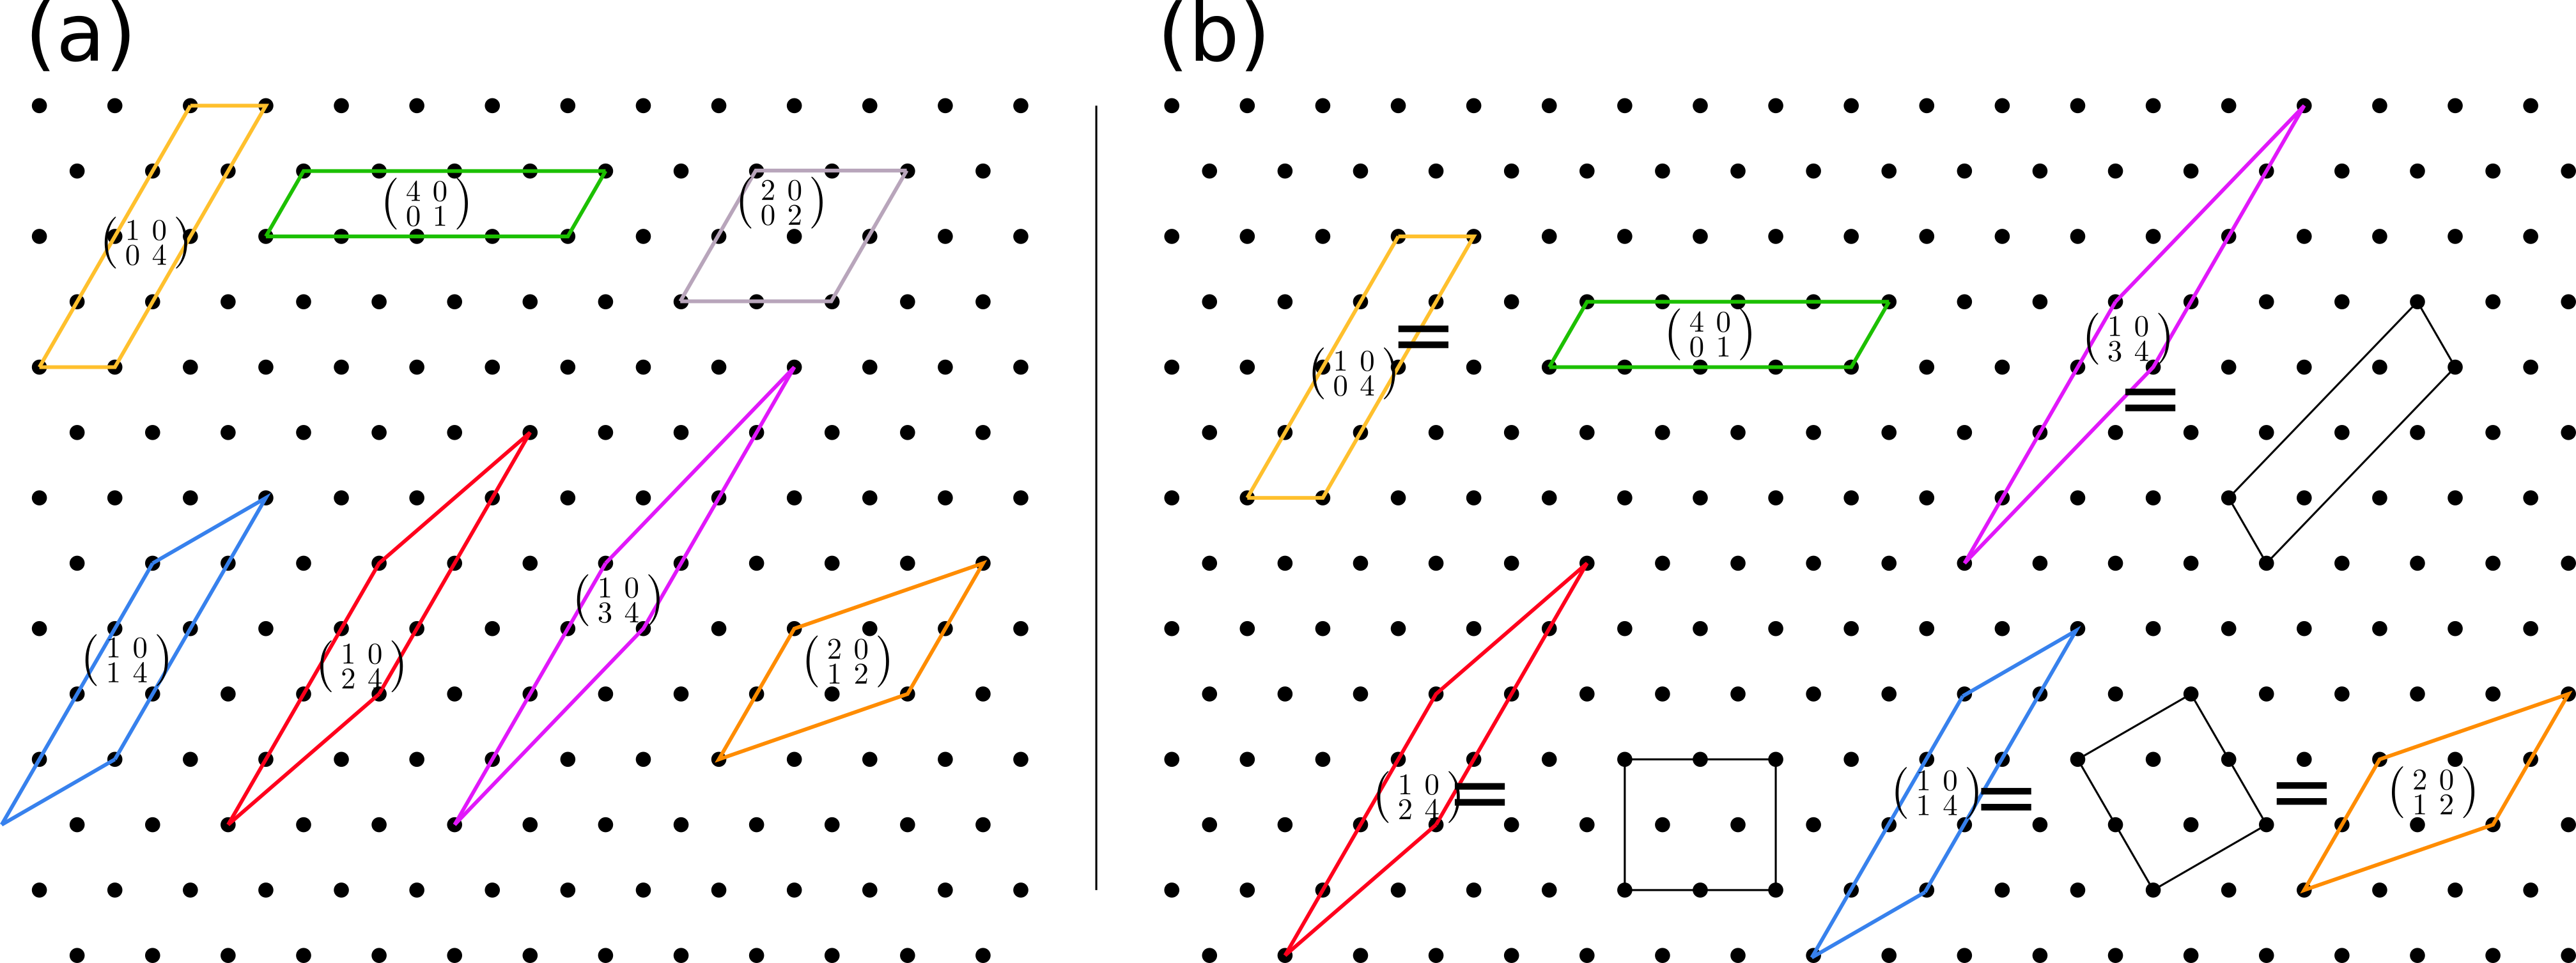
\includegraphics[width=0.96\textwidth]{figs/ch4_2d_tri_lattice.png}
  \centering
  \caption{三角格子晶格:(a) 7个大小为四倍原晶格的厄米标准型(HNF)基矢量及其对应的单位晶胞。(b)相同的超晶格,但使用最短的(正交的)基向量来描述。因此这七个二维晶格去重后可以得到完全不等价的超晶格。}
  \label{fig:ch4_2d_tri_lattice}
\end{figure}

在获取固定的超胞后,我们对硼原子进行替换,用一个过渡金属原子一次性替换两个三个或四个硼原子,
将过渡金属放在所替换的硼原子的空位的中心。
如图\ref{fig:ch5_how_cell_choose}所示阴影部分中的替代,共有三种方式,
分别对应替换两个,三个和四个硼原子,分别形成过渡金属与相邻硼原子配位数为八,
九和十的三种结构形式,我们将其初始结构分别命名为\rom{1}型\rom{2}型和\rom{3}型初始构型。

实际操作中,我们首先在\rom{1}型\rom{2}型和\rom{3}小结构单元的中心放置一个需原子,
以便后续进行过渡原子的放置。使用枚举的方法在所有可能的虚原子位置放置原子后,
使用中间处理过程,设置截断半径,用以去除过渡金属周围过近的硼原子,从而真正
实现使用一个原子半径较大的过渡金属替换由多个硼连接构成的结构小单元。
具体操作过程如图\ref{fig:btm3}所示。

\begin{figure}
  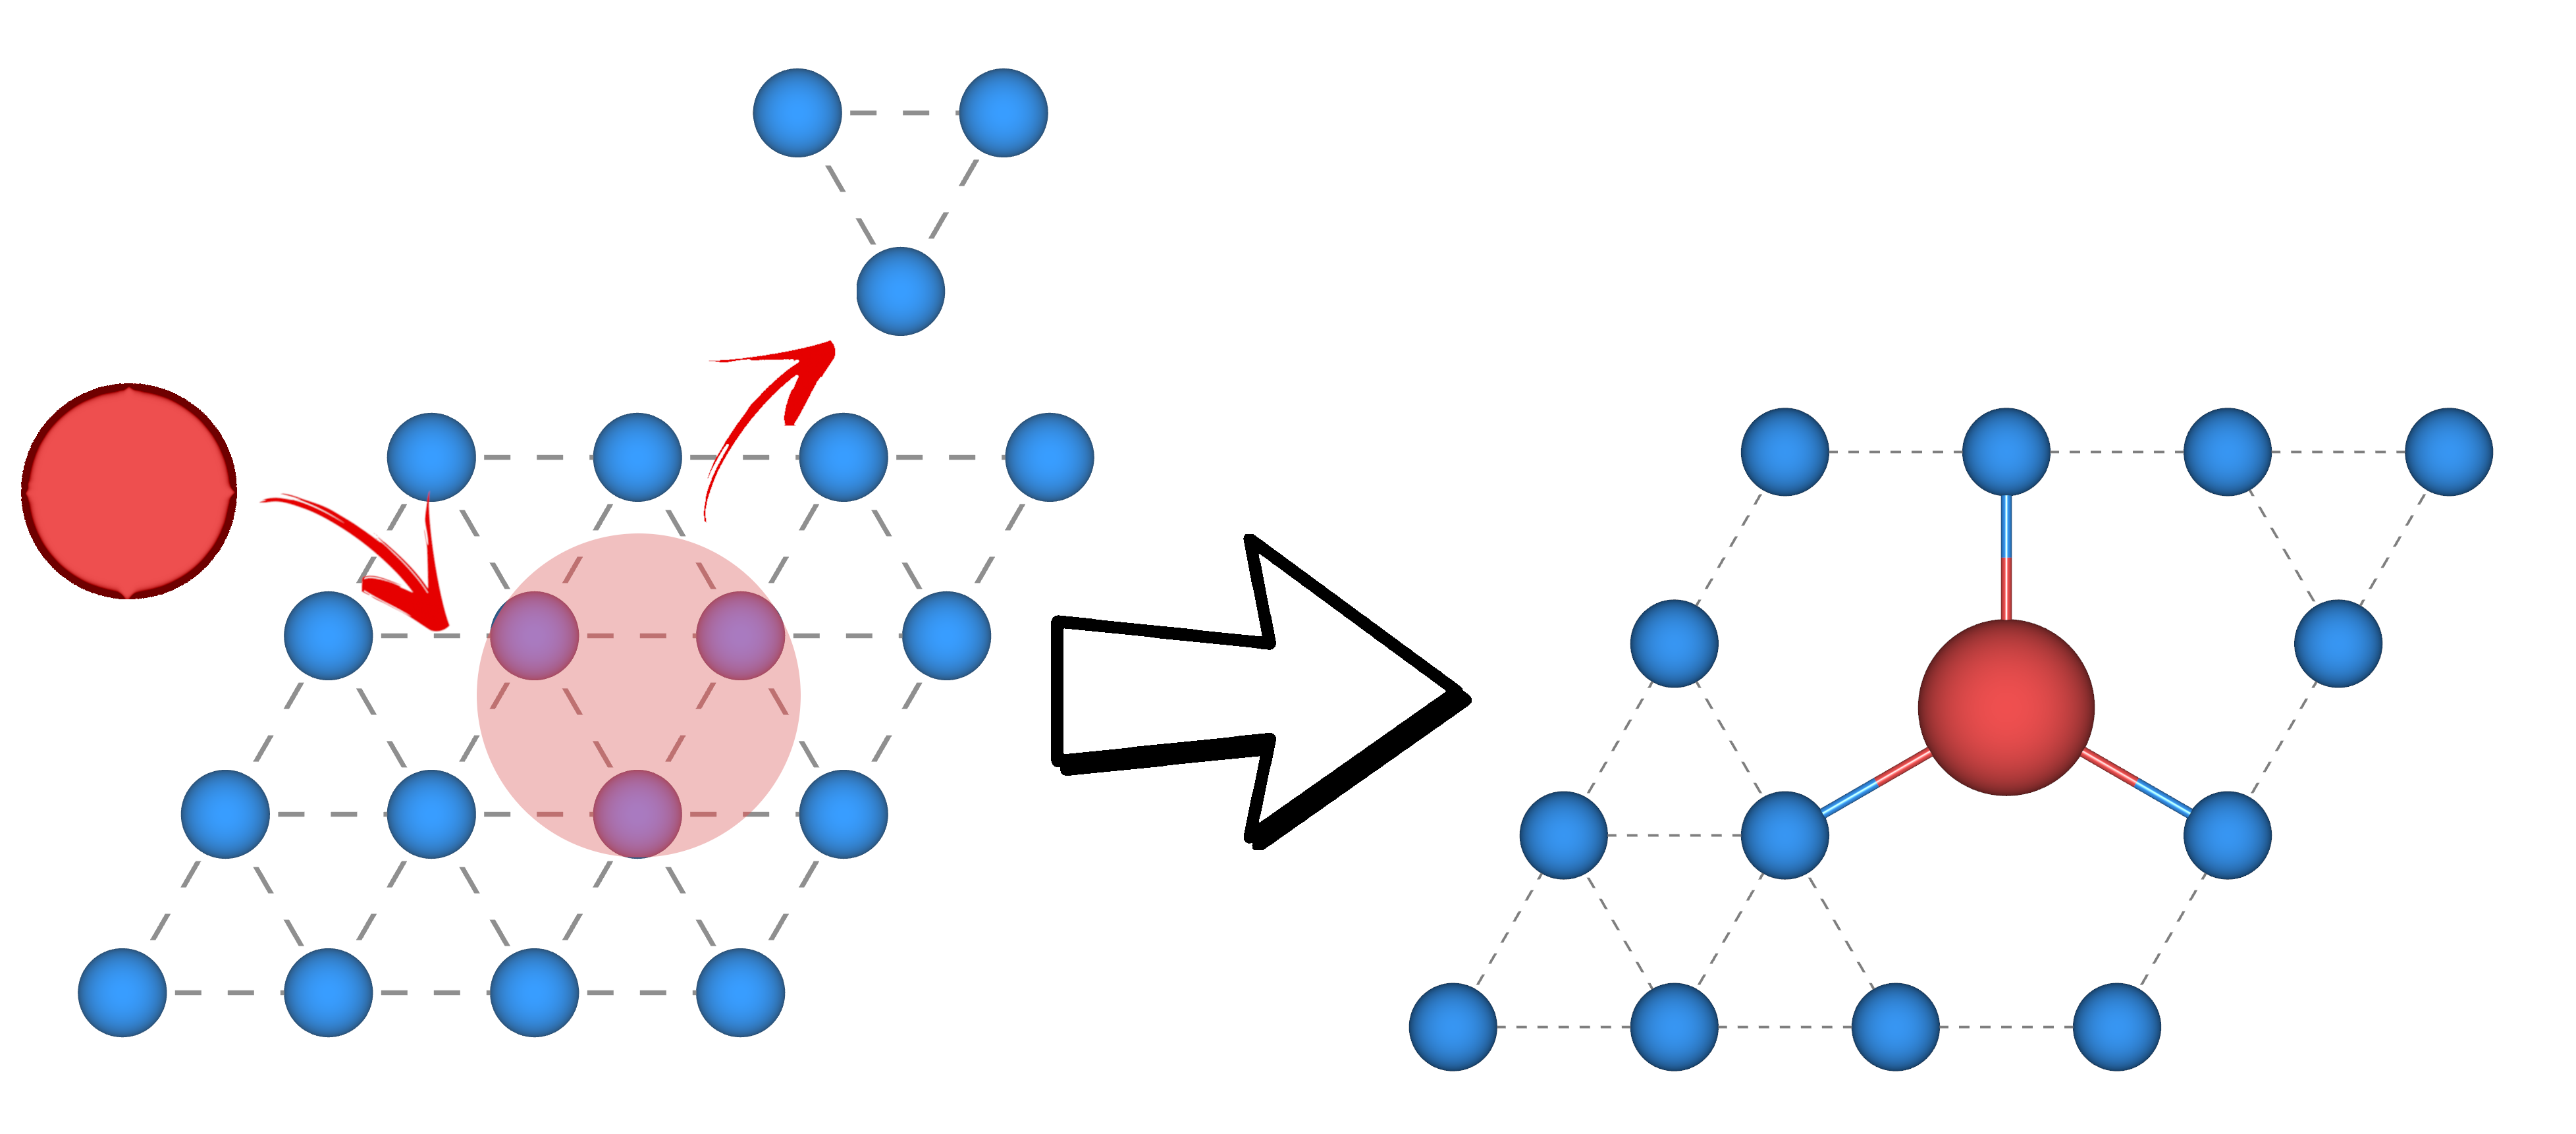
\includegraphics[width=0.96\textwidth]{figs/btm3.png}
  \centering
  \caption{用过渡金属原子替换\rom{2}型相连的硼原子的示意图。}
  \label{fig:btm3}
\end{figure}


替换后的构型会存在等价的构型,我们通过查重算法将等价的构型去除。
同时需要提到的是,根据已知经验,过渡金属应该与硼形成配位,
而金属-金属直接相连的结构能量上并不占优,为验证这个条件,我们在其中一个超胞下面的构型中,
测试了几个金属金属相连的生成构型,结果显示与相同化学计量的构型相比,其能量高出许多。

最后,通过以上步骤,我们一共获得了胞面积小于等于16个单胞的超胞下替换后的构型,
\rom{1}型\num{210}个,\rom{2}型\num{98}个,\rom{3}型\num{150}个。
这样的数量与全局搜索算法所需要的总数相比少了许多(全局搜索算法对特定原子数配比,
需要进行上千个结构的优化计算)。值得关注的是,
我们使用较少的计算量就能够发现各种不同配比下的全局搜索所能发现的全部单层稳定构型,
并还发现了能量比已经报导的更低的构型,这个结果我们将在下一节详细叙述。这种搜索策略高效的原因,
是因为我们在初始结构的生成中较好的应用了已知的结构上的样式特征,即硼三角网格的过渡金属硼形成多配位。

对上面提到的生成的钛硼原子比例从$1:2$到$1:13$的各种钛硼单层构型,在进行结构优化后,
我们还对其进行了能量和电子结构的高通量计算,并对每种钛硼原子比例下能量较低的构型分析了其超导电性。
相关内容将在论文的后两章详细描述。

\section{本章小结}

在这一章中,我们介绍了结构查重的完整算法和实现细节。
对特定晶格的衍生构型的高通量计算中,结构查重能够大大减少
所需要计算的构型数量,从而节约计算资源。
我们使用了HNF矩阵来表示不依赖于原始晶格、有限个的超胞的表示,进行晶格的查重。
% 通过对特定晶格使用HNF矩阵表示确定扩胞倍数的晶格,
% 利用Niggli将晶胞变换到标准形式,
再通过对称性给出特定晶格一定扩胞体积的所有不重构型,
从而可以快速地在构型查重中去除平移操作所导致的重复构型。

使用构型查重,我们生成并高通量计算了氟化石墨烯不同覆盖度下的可能构型
及其电子结构性质。结果显示F-graphene随覆盖度变化,
不同的构型会出现各种各样的能隙,且部分结构有较大的带隙,
揭示了F-graphene/Si器件有较宽的频率带宽的原因。
对于给定尺寸的单层硼化钛体系,我们考虑各种可能的超胞形状,
通过结构检查,生成了不重复的各种合理的初始构型,
以进行后续构型的进一步优化和性质的计算。

